\subsection[]{Driftkammer}

\begin{frame}{Driftkammer}
    \begin{columns}[T]
	    \column{.5\textwidth}
	    	\begin{itemize}
	    	  \item Messung der Ortsinformation durch Messung der Driftzeit
			  \item Aufbau: Proportionalzähler mit Trigger (Szintillator $\rightarrow$ schnelles Signal)
			  \item Trigger gibt den Zeitpunkt $t_0$, an dem Teilchen eintrifft
			\end{itemize}
			
	    \column{.5\textwidth}
	    	\begin{itemize}
			  \item Anode gibt den Zeitpunkt $t_1$, an dem Signal (Elektronen) eintrifft
			  \item bei bekannter Driftgeschw. $u$: Distanz von Enstehungsort zu Anode ist
			  $x=\int_{t_0}^{t_1}u\cdot dt$
			\end{itemize}
    \end{columns}

	\begin{figure}[htbp]
	  	\centering
		\includesvg[svgpath=bilder/, width=0.7\textwidth]{drift}
	  	\caption{Aufbau einer Driftkammer}
	\end{figure}
\end{frame}

\begin{frame}{Driftkammer}

	\begin{block}{Wie kommt die Spur zustande?}
		\begin{itemize}
		  \item mehrere Ebenen hintereinander, um Spur zu rekonstruieren
		  \item verschiedene Orientierungen der Drähte
		\end{itemize}
	\end{block}
	\vspace{0.8cm}
    \begin{columns}[T]
		\column{.45\textwidth}
			\textbf{Vorteile}		
			\begin{itemize}
			  \item großflächiger Aufbau möglich
			  \item wenige Kanäle
			  \item gute Ortsauflösung ($O(100\mu m)$)
			\end{itemize}	
	    \column{.5\textwidth}
	    	\textbf{Nachteile}
	    	\begin{itemize}
			  \item Größerer Abstand der Drähte $\rightarrow$ höhere Rate pro Draht 
			  \item hohe Ansprechzeit
			\end{itemize}
    \end{columns}
    \vspace{1cm}
\end{frame}

\begin{frame}{Driftkammer}
    	\begin{figure}[htbp]
				  \centering
				  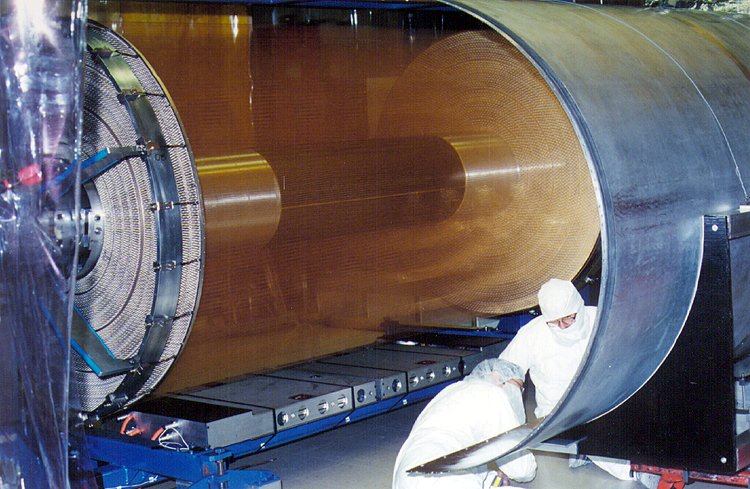
\includegraphics[scale=0.9]{bilder/beispiele/driftchamber.jpg}
		\end{figure}
		Driftkammer am BaBar Experiment, Stanford Linear Accelerator Center [gdc]:\\
		7104 Driftzellen (hexagonales Muster der Kathodendrähte)\\
		80 \& 120~$\mu$m Aluminium-Kathodendrähte, 20~$\mu$m Wolfram-Anodendrähte

\end{frame}